%!TEX root = ../main.tex

\section{Turning the problem around} % (fold)
\label{sub:turn_the_problem_around}

There are several ways to integrate general software tools in KBE development. One way, is to make the KBE tools adapt to the rest of software development environment. This way, all ready-made and future-make general software tools, can be used in KBE development without major adapting work. The KBE environment will naturally follow the evolution in software development, and can easily adapt to new changes. The KBE system vendor can focus on their core operation, and not spend time trying to adapt to the rest of the software evolution.

This idea is based one one key assumption, that it is easy to integrate general software tools in a KBE-system that is based on a general programming language. We will formulate this assumption as the following research question:

\begin{myrq}
\label{rq:intgenssofttools}
Is it easy to integrate general software tools, if a KBE-system is based on a widely used programming language?
\end{myrq}

\subsection{How to test the hypothesis?} % (fold)
\label{ssub:how_to_test_our_hypothises}
In order to begin to answer this question, we have to overcome one notable obstacle. As of today, there is no KBE-system that follows the general software evolution. The major KBE-systems use proprietary languages like GDL, IDL and AML. These languages are highly adapted for KBE development, but lack the great support that widely used languages have. To investigate this question, we therefore have to make a minimal KBE-system based on a general software language. Only then we can test our hypothesis.

We will therefore make a minimal KBE-system based on Python, Open CASCADE and FreeCAD. Then we will investigate if it is easy to integrate some of the general software tools that Python supports.
% subsubsection how_to_test_our_hypothises (end)


\subsection{The minimal KBE system} % (fold)
\label{sub:the_kbe_system}
In order to make a minimal KBE-system, we must understand the core features of a KBE system, and how this can be implemented. Rocca et al. investigates this as a part of the paper: \enquote{Knowledge based engineering: Between \{AI\} and CAD. Review of a language based technology to support engineering design'} \cite{rocca}. Rocca argues that a basic KBE-system contains three essential parts, a viewer, geometry kernel and a programming interface, as shown in figure \ref{fig:3parts}.

\begin{mydef}
  A minimal KBE system is build up of a geometry kernel, graphical viewer and a programming interface.
\end{mydef}

\begin{figure}[ht!]
\centering
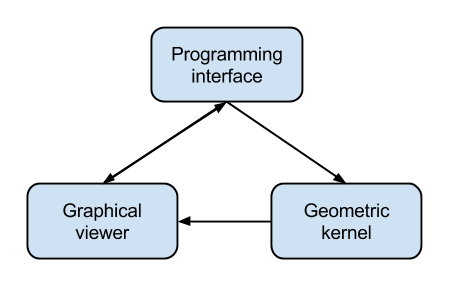
\includegraphics[width=90mm]{gfx/kbe_system_in_3_parts.png}

\caption{The tree essential parts in a KBE-system and their relation}
\label{fig:3parts}
\end{figure}

\begin{description}
  \item[The programming interface] is what makes a KBE-system special. This is where the rules governing each model is stored. It also describes the object structure needed to create the geometry. The programming interface is build up of a programming language, and must have an interface to the geometric kernel. It must also communicate with the viewer, so the viewer knows about each KBE-object, its parameters and the relation between each object.
  \item[The graphical viewer] is where the KBE-object and models can be queried and visualized. The are often tree main components.
  \begin{description}
    \item[The tree pane] shows the object hierarchy.
    \item[The inspector pane] is where the properties of a KBE-object can be viewed and manipulated.
    \item[The view-port pane] is where the KBE-model is visualized.
  \end{description}
  \item[The geometric kernel] is a 3D modeling component, which feed geometric data to the viewer, based on data received by the programming interface module.
\end{description}

The main feature of a KBE system is the programming interface. The programming interface governs the object structure, logic and control that can be implemented in the KBE model. The two other components, the graphical viewer and geometric kernel, is used in many engineering systems today and is not a unique KBE part. Many CAD systems, like NX UGS, FreeCAD and AutoCAD, use the same combination, but the KBE viewer differs in how it visualize a models meta data, and the control components. The viewer system of a KBE system and a CAD system is still comparable.
% subsection the_kbe_system (end)


\subsection{Programming interface} % (fold)
\label{sub:programming_interface}
To make a minimal KBE-system, we must first choose a suitable programming language. Today almost all KBE languages are object oriented and have some main declaration types, as shown in Table~\ref{tab:languageParts} from \cite{rocca}. Possibly the most relevant operator is the \texttt{define-class}operator, which declares a class definition. It allows defining classes, superclasses, objects and relationships of inheritance. We can organize the rest of the expressions, as ether attribute function or subclass declarations. The attributes can again be divided in default, descendant, editable or normal attributes declarations. These declarations are similar to the modern object-oriented programming paradigm, which is supported by many general purpose programming languages today. The basic concept for this paradigm, is to represent the consent of objects with attributes and methods and the relationship between these objects \citep{van_ray}s.

\begin{table}[ctb]
  \begin{center}
    \begin{tabular}{p{4cm}lp{5cm}l}
    \hline
    \textbf{GDL} & \textbf{IDL} & \textbf{Knowledge Fusion} & \textbf{AML} \\
    \hline
      define-object & defpart & defclass & Define-class \\
      input-slot & input & Any data type a followed by the behavioral flag b parameter (plus optional default value)&\\
      Input-slot:settable (or:defaulting) & Default-inputs&&\\
      computed imputs& attributes&Specification of several data types, plus an optional behavioral flag(e.g., lookup, uncached and parameter) &\\
      computed-slot:settable  &Modifiable-attributes&A data type followed by the behavioral flag modifiable&\\
      Trickle-down-slots &Descendant-attributes&All attributes descendant by default&\\
      Type &Type&Class&\\
      Objects&Parts&Child&Sub-objects\\
      Hidden-objects &Pseudo-parts& Class name starts with&\\
      Functions &Methods&Functions&\\
    \hline
    \end{tabular}
  \end{center}
  \caption{KBE language operators to define classes and objects hierarchies}
  \label{tab:languageParts}
\end{table}


\subsubsection{Essential features} % (fold)
\label{ssub:essential_features}
We see that the basic concepts of a KBE language is supported in the object-oriented paradigm \citep{rocca} with one exception. The specific attribute declaration, which describe how the attribute should be handled throughout the instantiation and inheritance procedure, is not a standard feature of most general purpose object-oriented languages. This features is handled by native declarations in most KBE languages, but this might not be a necessary feature. Controlling instantiation and inheritance procedure can be handled by creating a basic object structure. The basic object structure can then control relations like superclasses and children in the object hierarchy. It can also make the different types of attributes.

Other essential part of a KBE language, is its ability to give commands to a geometric kernel. To make this possible, an interface have to exist between the language and the geometric kernel.
% subsubsection essential_features (end)


\subsubsection{Non-essential features} % (fold)
\label{ssub:non_essential_features}
Some features make the KBE language more more flexible and controllable, but is not essential. Dynamic typing and multiple inheritance are two examples. Languages without these features are more strict, and don't support mixins, which, for example, make implementing materials and coordinate systems easier. Knowledge Fusion is one kind of KBE language that don't support these features \citep{rocca}.

Models also tend to be very large when making KBE application, which make calculation and rendering of the model time consuming. This is solved by many KBE-systems today with demand driven evaluation. Demand driven evaluation, also known as lazy evaluation, is an evaluation strategy, which delays the evaluation of an expression until its value is needed. This gives the KBE system the ability to just recalculate and render the parts needed in the model update. There are more solutions to this problem than just a native support for lazy evaluation. One solution is to implement a pattern called observable pattern. This pattern allows a one-to-one or one-to-many dependency between objects, so that when the observed object is changed in some way, all the observers can be notified \citep{rollings}.

Other notable non-essential features, are syntactic overhead and open source. Syntactic overhead is a programming languages ability to eliminate syntactic elements, unnecessary in a given problem domain. The \enquote{Hello World} example in Java exemplifies syntactic overhead. The developer has to contain the print statement in an main function and a container class, none of which serves the overarching goal of printing a string to the console. For this problem domain, printing a string to the console, Java would be considered to have high syntactic overhead. This is not always a bad feature, but using a programming languages with low syntactic overhead can mean less writing and more focus on the essential parts of the model. The benefit of open source programming languages, is that widely used open source languages often get a lot of constructive feedback from the open source community regarding bug reports and fixes, support, development of new software tools and libraries, as well as a collaborative culture. This often leads to programming languages with high quality, good documentation and a wide variety of support tools.

\begin{mydef}
  Syntactic overhead is a language ability to eliminate unnecessary syntactic elements for a given problem domain.
\end{mydef}
% subsubsection non_essential_features (end)


\subsubsection{Choosing a programming language} % (fold)
\label{ssub:choosing_a_programming_language}
We can review some key features from the discussion above, and try to evaluate what kind of programming languages that are suitable for KBE development. The result of this evaluation is shown in Table~\ref{tab:chooselanguage}. We have chosen to spit the features in essential and non-essential features. The essential features are that we regard as a \enquote{must have} feature, while non-essential features are \enquote{nice to have}. We also added one other category, which try to describe what kind of general software tools that is supported in the programming language.

\begin{table}[tb]
  \begin{center}
    \begin{tabular}{|l|c|c|c|c|c|c|}
    \hline
     \textbf{Feature}& \textbf{AML} & \textbf{Python} & \textbf{CLisp} & \textbf{C}++  & \textbf{C}\# & \textbf{Java} \\
    \hline
       \multicolumn{7}{ |l| }{\textbf{Essential features}} \\
    \hline
    Object-oriented & Yes&Yes&Yes&Yes&Yes&Yes\\
    \hline
    Interface to geometric kernel & Yes&Yes&Yes&Yes&Yes&Yes\\
    \hline
    \multicolumn{7}{ |l| }{\textbf{Non-essential features}} \\
    \hline
    Native demand driven evaluation & Yes&Yes&Yes&No&Yes&No\\
    \hline
    Dynamic typing & Yes&Yes&Yes&No&No&No\\
    \hline
    Multiple inheritance & Yes&Yes&Yes&No&No&No\\
    \hline
    Open source & N&Yes&Yes&Yes&No&Yes\\
    \hline
    Syntactic overhead & Low&Low&Low&High&Medium&Medium\\
    \hline
    \multicolumn{7}{ |l| }{\textbf{General software tools}}\\
    \hline
    Debugging tool &No&Yes&Yes&Yes&Yes&Yes\\
    \hline
    Test framework support &Low&High&Medium&High&High&High\\
    \hline
    IDE support &Low&High&Medium&High&High&High\\
    \hline
    Community &Low&High&Medium&High&High&High\\
    \hline
    \end{tabular}
  \end{center}
  \caption{A comparison table between KBE language features and some programming languages.}
  \label{tab:chooselanguage}
\end{table}

From Table~\ref{tab:chooselanguage} we can draw some conclusions. First we see that all languages is a suitable KBE language, because they all support the essential features. The specific KBE object structure and hierarchy is something that all the languages can imitate. When we look at the non-essential section, we see that some languages are more suitable than others. Common Lisp, AML and Python stand out as the three most suitable languages. They have all the features that enhance flexibility and control, like demand driven evaluation, dynamic typing and multiple inheritance. They also have a low syntactic overhead. Another ting that differentiates them is that they are open source.

Investigating the feature most relevant to our RQ~\ref{rq:intgenssofttools}, the GSD tool support, we observe that Python, C++, C\# and Java has the most support. All languages have a good and varied selection of compatible general software tools, and this makes them highly selectable for our test. The loser in this category is AML, probably due to this being a lesser used, proprietary programming language. A honorable mention is the AUnit test framework for AML, but this tool is still in development.

Based on this evaluation we choose to use Python as our base language, because it has all the features needed to become a KBE language, and has good support for general software tools, which is crucial in order to explore our research question.
% subsubsection choosing_a_programming_language (end)
% subsection programming_interface (end)


\subsection{Geometric kernel and graphical viewer} % (fold)
\label{sub:geometric_kernel_and_graphical_viewer}
A programming language alone does not make a KBE system. We still need to find a geographical viewer and a geometric kernel. Available modeling kernels compatible with Python are:

\begin{itemize}
  \item \textbf{Parasolid} by ShapeData, now owned by Siemens.

  \item \textbf{ACIS} by Spatial Corporation.

  \item \textbf{ShapeManager} by AutoDesk.

  \item \textbf{RGK} by Russian Federation's Ministry of Industry and Trade.

  \item \textbf{Open CASCADE} - by open source community.
\end{itemize}

The two most used kernels are Parasolid and ACIS, which are use by NX, AML, AutoCAD and SpaceClaim. RGK is a newly developed kernel, with a lot of positive feedback \citep{RGK}, but is still in development. The only major geometric kernel that is both proven in other applications and based on open source, is Open CASCADE and is therefore the only one economic scope of this project. It includes C++ components for 3D surface and solid modeling, visualization and data exchange.

The geometric kernel and graphical viewer has to be connected to each other and the programming language. This give some restriction in choosing the viewer component of our KBE system, since we have chosen Python as the base programming language. We are also restricted regard to development time, so a ready-make viewer and geometric kernel combination is preferable. Some open source applications satisfies our requirements:

\begin{itemize}
  \item The first option is PythonOCC \citep{OCC}. PythonOCC is an 3D CAD/CAE/PLM development framework for Python. There is no GUI component, just a Python interface to the underlying OpenCascade kernel and libraries to prototype a viewer.

  \item The second option is FreeCAD \citep{FreeCAD} and its Python objects called PytonFeatures. PythonFeatures are 100\% Python objects, and contains a visualization and geometry part. FreeCAD is a parametric 3D modeler. This makes it more similar to traditional CAD applications than PythonOCC. FreeCAD includes a built-in Python interpreter and an open API, that covers almost all features of the application. With this scripting feature, a developer is able to create an object structure, on top of the viewer and kernel, to create a KBE model.
\end{itemize}

Both these alternatives are able to give us the base of our testing platform. Both have a viewer and a geometric kernel, that is controlled by a Python API. All that is left, in order to create a KBE-model, is to create the programmable interface. Out of these two alternatives we choose FreeCAD. The main reason for this was development time, and since we only need a minimal KBE system to test our resource question (RQ~\ref{rq:intgenssofttools}), FreeCAD was the easiest application to use.
% subsection geometric_kernel_and_graphical_viewer (end)


\subsection{Creating the testing platform} % (fold)
\label{sub:the_creating_the_testing_platform}
Now we have the basic tools to create our testing platform. Before we start implementing, we need to set some restrictions on our minimal KBE system. There is no need to create a complete system to test our hypothesis, just the basic functionality.

\begin{itemize}
  \item Performance is not an issue, because we only need to make small models. Therefore we do not need to think about demand driven evaluation or other performance enhancing features.

  \item Only focus on geometry, not meshing or FEM analysis.

  \item Create a basic object structure, that support multiple inheritance and children.
\end{itemize}
% subsubsection restricting_the_test_platform (end)


\subsubsection{The object structure} % (fold)
\label{ssub:the_object_structure}
To control instantiation and relationship between each object, we have created a superclass, called KbePart (see Appendix~\ref{app:kbepart.py}). This object has to be inherited from all KBE classes. It contains a set of functions that can be used by the inherited classes, as described below.

\begin{description}
  \item[make\_properties()]  can be extended to add properties to the model.

  \item[make\_property(name, property\_type)] can be used to make a editable and descendant property. It returns a object with all editable and descendant properties.

  \item [add\_children()] is used to add and manipulate children.

  \item[make\_child()] is used to add a child.

  \item[get\_properties\_list()] return a list of all editable and descendant properties.

  \item[print\_msg()] can be used to print messages to the viewer's console pane.
\end{description}

\begin{figure}[ht!]
\centering
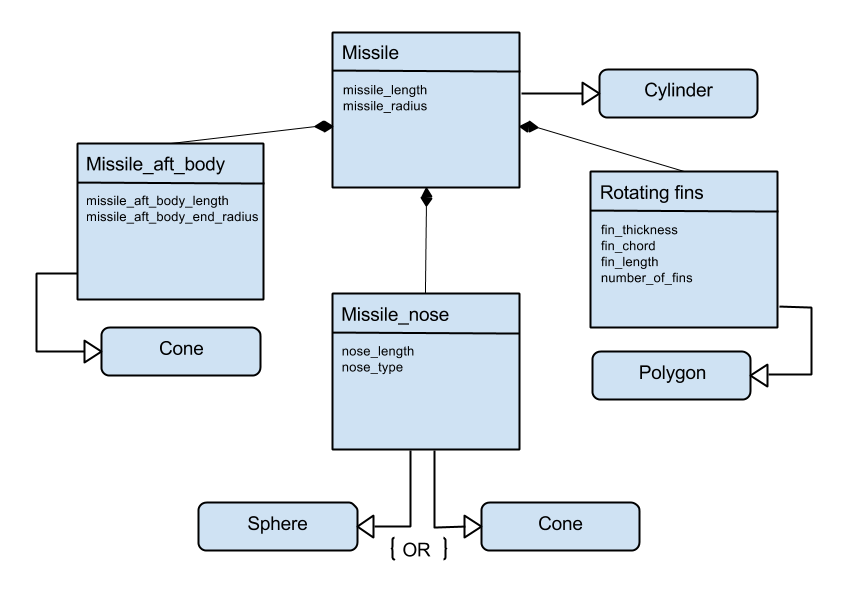
\includegraphics[width=150mm]{gfx/uml_diagram_of_missile.png}

\caption{UML Class diagram for the Missile class showing inheritance and composition links.}s
\label{fig:object_structure}
\end{figure}
% subsubsection the_object_structure (end)


\subsubsection{The test model} % (fold)
\label{ssub:the_test_model}
Based on this object structure, we have created a simple missile model (see Appendix~\ref{app:missile.py}), based on the case from the AML Basic Training Manual \cite{aml_ref}. This model is going to be used to test-environment for our hypothesis. The missile is build out of objects inherited from the KbePart. From figure~\ref{fig:object_structure}, we can see that the missile class is based on a set of other subclasses, missile\_nose, missile\_aft\_body and rotation\_fins.

From figure~\ref{fig:freecad}, we can see the graphical viewer with the three pane, editable properties pane and view-port pane. From the properties pane, we can see that all the properties have propagated from the child objects to the missile. The properties can also be edited to change the geometry of the missile.
% subsubsection the_test_model (end)
% subsection  (end)


\subsection{Integrating general software tool} % (fold)
\label{sub:integrating_general_software_tool}

Now that we have a test platform we can start integrating some general software tools. Three GSD tools, that are going to be investigated in particulare is debugging tools, tools for testing and IDE/editor support.


\subsubsection{Interfacing with FreeCAD and Open CASCADE} % (fold)
\label{ssub:Interfacing with FreeCAD}

To get Pythons general software tool to work in a FreeCAD environment, an interface need to exist between them. This interface is the Python programming language. All FreeCAD features, like modeling, meshing and simulations, are accessible thought a Python API. This makes it easy to integrate different kinds of tools. FreeCAD is imported into Python as a normal module. The process for doing this in a temporary way is shown below:

\begin{python}
import sys sys.path.append("path/to/FreeCAD/lib")
\end{python}

FreeCAD can now run inside other applications that use Python or from an external Python shell. We can also import our KbePart the same way:

\begin{python}
import KbePart
\end{python}

This makes our minimal KBE system very modular.

\begin{figure}[ht!]
\centering
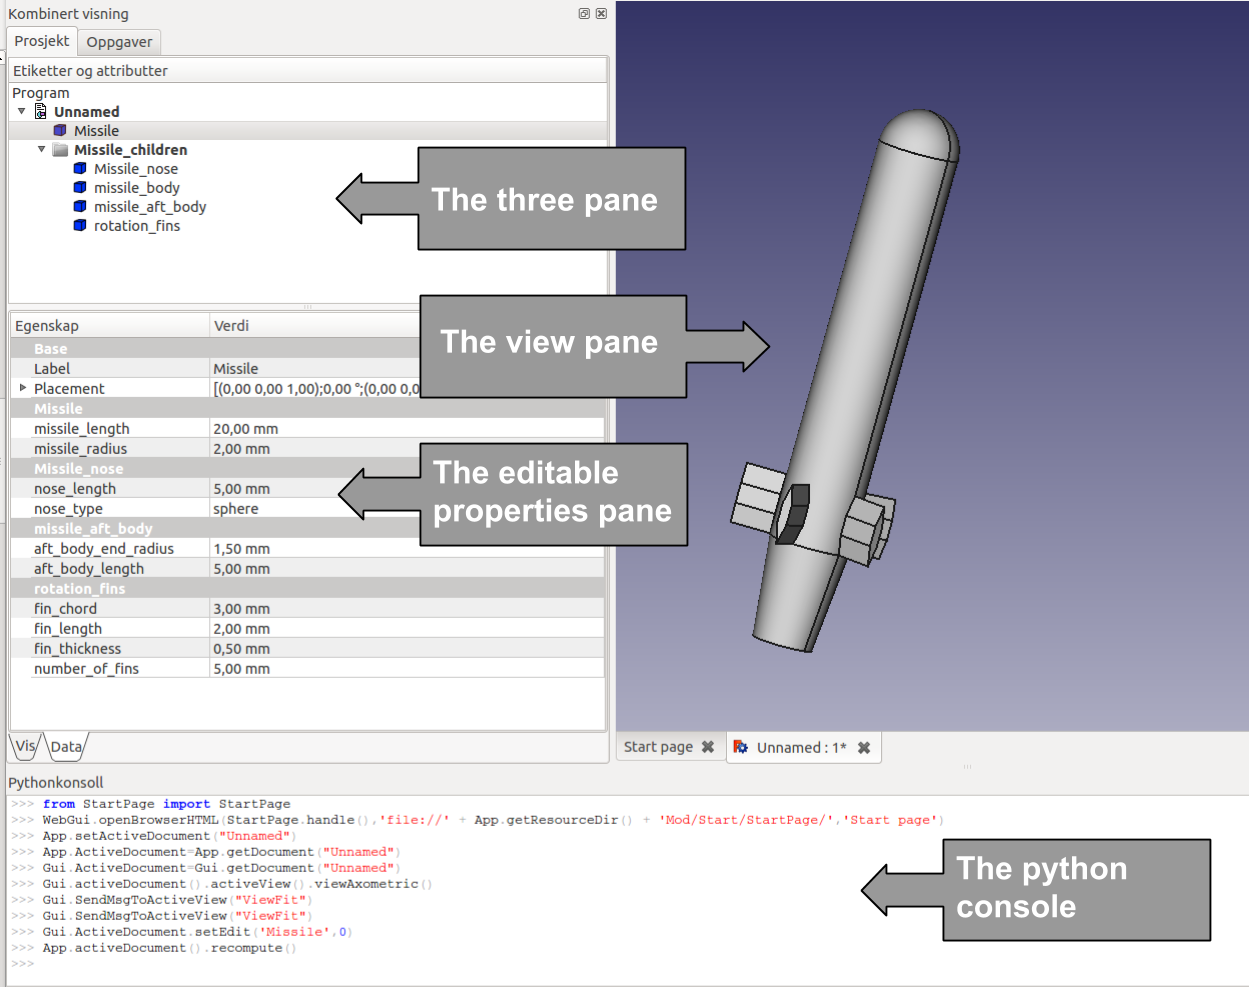
\includegraphics[width=120mm]{gfx/freecad_visulization.png}

\caption{The freeCAD graphical viewer visualizing the missile, with the three pane, editable properties pane, view-port pane and a Python console}
\label{fig:freecad}
\end{figure}
% subsubsection interfacing_with_aml_from_the_console (end)


\subsubsection{Testing support} % (fold)
\label{ssub:testing_support}
Testing is the practice of making objective judgments regarding the system's quality and correctness. It is a huge help for maintaining and developing a code base \citep{agile_samurai}. Testing big and complex structures, like KBE models, are not a easy task. Many problems tend to arise, because the different objects in the system have many complex dependencies between them \citep{aunit}. In the software industry this is solved with good testing frameworks and mocking. Mocking is done my creating mock objects, which are injected to isolate different objects from each other during testing. Mock objects are simulated objects that mimic the behavior of real objects in controlled ways. By using mock objects, we can assure that errors in one object does not affect the test results for another object. This makes locating errors and writing tests easier on complex systems, like KBE models.

Integrating a test framework in a KBE system, means that we have to isolate the models and their logic. In our case this implies we have to isolate the KbePart objects. They alone, hold all logic and rules governing the model and their geometry. With KbePart being a complete Python module, it is easy to integrate any test framework supported by the Python programming language.

Python have a large variety of test frameworks to choose from. Some varieties are unittest, pyUnit, py.test or doctest. They all have positive and negative qualities. We have chosen unittest, as this is the currently most used testing framework for Python.

Integrating the unittest framework was done in a normal manner. We imported the module and created a test case class.

\begin{python}[caption={Creating a TestCase},label={lst:test_case}]
  import unittest
  from mock import Mock

  class DescribeMissile(unittest.TestCase):

    def setUp(self):
        self.missile_doc = DocumentMock()
        self.missile = Missile(self.missile_doc)
        self.fp = FeaturePythonMock()
\end{python}

The \textit{setUp} function is called before each test is executed. We make the missile from independent from its dependencies, by creating two different mock objects, as we can see from the code snippet above and in Appendix~\ref{app:missile_spec.py}. The document mock simulates the freeCAD document where every model is added. The FeaturePythonMock is an object that represent all properties, so we can control them in the test situation. Every KbePart have control of its own objects, making it easy to abstract the parts currently being tested. Now we can start to make some tests. The first test, shown in Listing~\ref{lst:test_1}, is checking if the missile has four children.

\begin{python}[caption={Missile test 1},label={lst:test_1}]
   def test_missile_should_be_init_with_4_children(self):
        children_length = len(self.missile.children)
        self.assertEqual(children_length, 4)
 \end{python}

We are also able to mock out the objects/attributes/functions we want. Listing~\ref{lst:test_2} shows how we have mocked out the missile's execute function.

\begin{python}[caption={Missile test 2},label={lst:test_2}]
    def test_missile_should_update_when_a_value_is_changed(self):
        self.fp.missile_radius = 5
        self.missile.execute = Mock(return_value=True)
        self.missile.onChanged(self.fp, 'missile_radius')
        self.assertTrue(self.missile.execute.called)
\end{python}
% subsubsection testing_support (end)


\subsubsection{Debugging support} % (fold)
\label{ssub:debugging_support}
A lot of different debugging tools are available for the Python programming language. Some examples are WinPDB, PyDebug which are embedded in many Python IDEs. The most basic debugger is the Python debugger, which is available as a Python module called pdb. At the core this is a command line debugger, but there exists graphical interface that work with it. It also integrates with the Sublime Text 2 editor. It is integrated just by importing the pdb module. A breakpoint as created by inserting a \textit{pdb.set\_trace()}. When the code is executed, the developer is free to access all the debugger features through the command palette in Sublime, see Figure~\ref{fig:sublime_ide}.
% subsubsection debugging_support (end)

\subsubsection{IDE support} % (fold)
Many IDE options exist for Python. Some of the most acclaimed are PyCarm, Eclipse with PyDev, Wing and Sublime Text. We chose to integrate our it in sublime text, since it is our favorite editor, has a great variety of features and makes a nice comparison to our Sublime AML integration.

To better configure Sublime to Python editing, the anaconda \citep{anaconda} plug-in should be used. Anaconda adds a wide spectrum of facilities, like auto-complete, goto definition, goto documentation, refactoring, linting and much more. It also adds a lot of handful snippets.

To integrate Python debugger, the plug-in SublimeREPL was used. SublimeREPL is able to run a Python interpretor in a Sublime buffer. SublimeREPL has a command to run current file in pdb-mode, which is useful for debugging.

Sublime supports unit-testing out of the box. \textit{Ctrl+b}, compiles and runs the current test file. A little buffer at the bottom of the editor will pop up and display the test results, as shown in Figure~\ref{fig:sublime_ide}.

\begin{figure}[ht!]
\centering
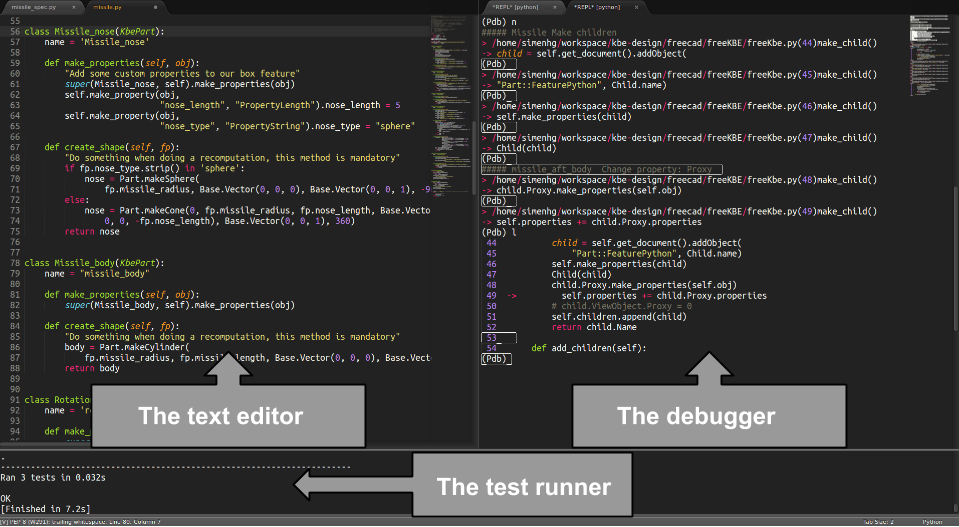
\includegraphics[width=120mm]{gfx/sublime_ide_arrows.png}

\caption{Sublime text integration, displaying the test runner, the debugger and the text editor.}
\label{fig:sublime_ide}
\end{figure}
% subsubsection ide_support (end)
% subsection integrating_general_software_tool (end)


\subsection{Problems with switching KBE-system} % (fold)
\label{sub:problems_with_switching_KBE_system}
In this chapter we have created a minimal KBE system and integrated a set of general software tools. In our tests, no major obstacles have been encountered. However, this is not conclusive evidence that creating a new KBE-system is an easy task.

Despite the fact that creating a new KBE System seems like a easy solution, some major problems has to be solved. One problems is continuation of knowledge. Today all knowledge and logic connected to a KBE model is interleaved in the KBE classes. This means that all knowledge is lost if one decide to switch KBE system. The knowledge can, however, be transferred to a new KBE system. It can for example be done by parsing the objects to the new system. It should be said that this is not an easy task and should be examined before attempting to create a new KBE system.

Time and quality is also factors we need to take into account. Although it is easy to integrate general software tools in a new KBE system, it may not be the best solution. The time it takes to create a good KBE system may exceed the time to integrate general software tool. The quality of a new system may also not be as good as a old and fully tested system.
% subsection problems_with_switching_KBE_system (end)
% section building_a_KBE_system (end)
